\section{Vorbereitungsphase}
Die Arbeiten am Projekt begannen mit der Vorbereitungsphase. Das Zeil dieser war es, wichtige Abklärungen zu machen und Entscheidungen zu treffen damit im ersten Sprint mir der eigentlichen Entwicklung begonnen werden konnte.
Dies beinhaltete zum einen eine Befragung potenzieller Benutzer der zu entwickelnden Applikation sowie die Evaluation eines geeigneten Technologiestacks.
Mit einer Dauer von zwei Wochen war die Vorbereitungsphase gleich lang, wie ein Sprint. Bei ihr handelt es sich jedoch nicht um einen richtigen Sprint, da noch kein Backlog mit User Stories vorhanden war.
Der Backlog für die Sprints wurde währen dieser Phase basierend auf den Erkenntnissen der zuvor genannten Punkte erstellt.
In den folgenden Abschnitten wird die Umsetzung der Vorbereitungsphase detailliert beschrieben.

\subsection{DlmsQuickAccess}
Für die Erstellung des Projekts in \ac{ADO}, für das Git-Repository sowie für die C\# Solution wurden jeweils Namen benötigt.
Dazu wurde \textit{DlmsQuickAccess} kreiert.
Der Name ist an die zu ersetzende Funktion des \ac{DMT2}, \textit{Quick Access}, angelehnt.

\subsection{Nutzerbefragung}
Wie im Kapitel \ref{erwarteteResultate} erklärt, ist das Ziel dieses Projekts, die bestehende Anwendung, \textit{DMT2}, durch einen Neuentwicklung zu ersetzen.

Am Standort Cham der Landis+Gyr gibt es zwei Entwicklerteams, welche den DMT2 regelmässig verwenden.
% TODO öppis zu dene Teams schriibe, Hinweis, der Autor dieser Arbeit ist ebenfalls teils eines dieser Teams
Für dieses Projekt wurden die Mitglieder dieser beiden Teams als Nutzer definiert und in dieser Arbeit so bezeichnet.  % chamer das besser formuliere?
Zu Beginn der Vorbereitungsphase wurden alle Nutzer zu einem Meeting eingeladen.
In diesem Meeting wurden erörtert, welche Dinge bei der bestehende Anwendung bereits gut funktionieren und welche als störend wahrgenommen werden.
Ebenfalls wurde von den Nutzern Ideen \& Wünsche für die Neuentwicklung abgeholt.

Für das sammeln der Antworten wurde während des Meetings retrotool.io TODO eingesetzt.
Die Abbildungen \ref{fig:WhatWorksWell}, \ref{fig:WhatBothersYou} und \ref{fig:IdeasAndWishes} sind Screenshots daraus.

% todo In einem anderen Kapitel die Resultate der Umfrage aufarbeiten und hier referenzieren
% https://retrotool.io/8mWyxCzpbIfQPydp2FPf4


\begin{figure}[H]
   \centering
   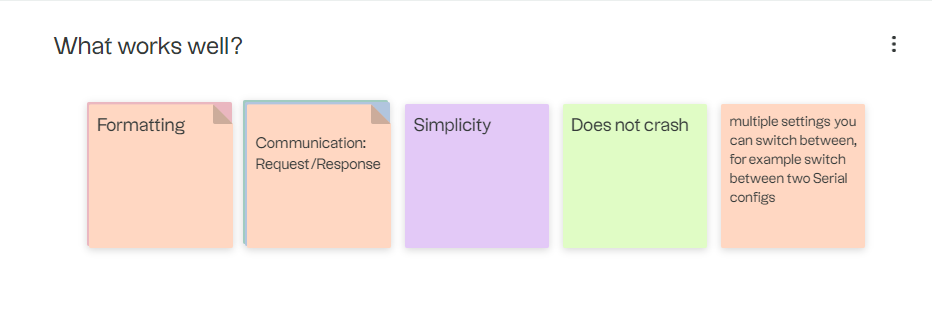
\includegraphics[width=1.0\textwidth]{gfx/S1_RetroBoard_WhatWorksWell.png}
   \caption{
       Antworten der Nutzer zur Frage "Was funktioniert bereits gut?"
   }
   \label{fig:WhatWorksWell}
\end{figure}

\begin{figure}[H]
   \centering
   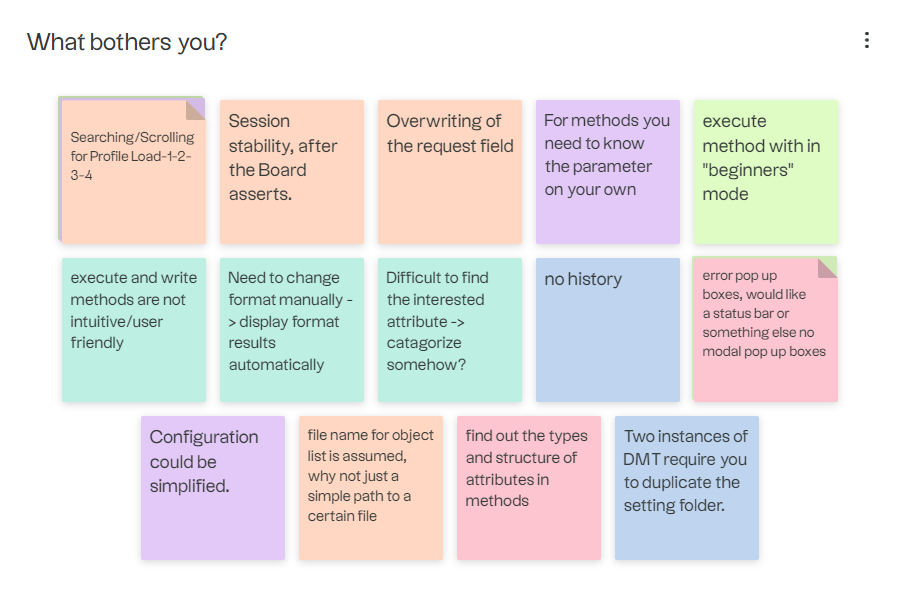
\includegraphics[width=1.0\textwidth]{gfx/S1_RetroBoard_WhatBothersYou.png}
   \caption{
       Antworten der Nutzer zur Frage "Was stört dich?"
   }
   \label{fig:WhatBothersYou}
\end{figure}

\begin{figure}[H]
   \centering
   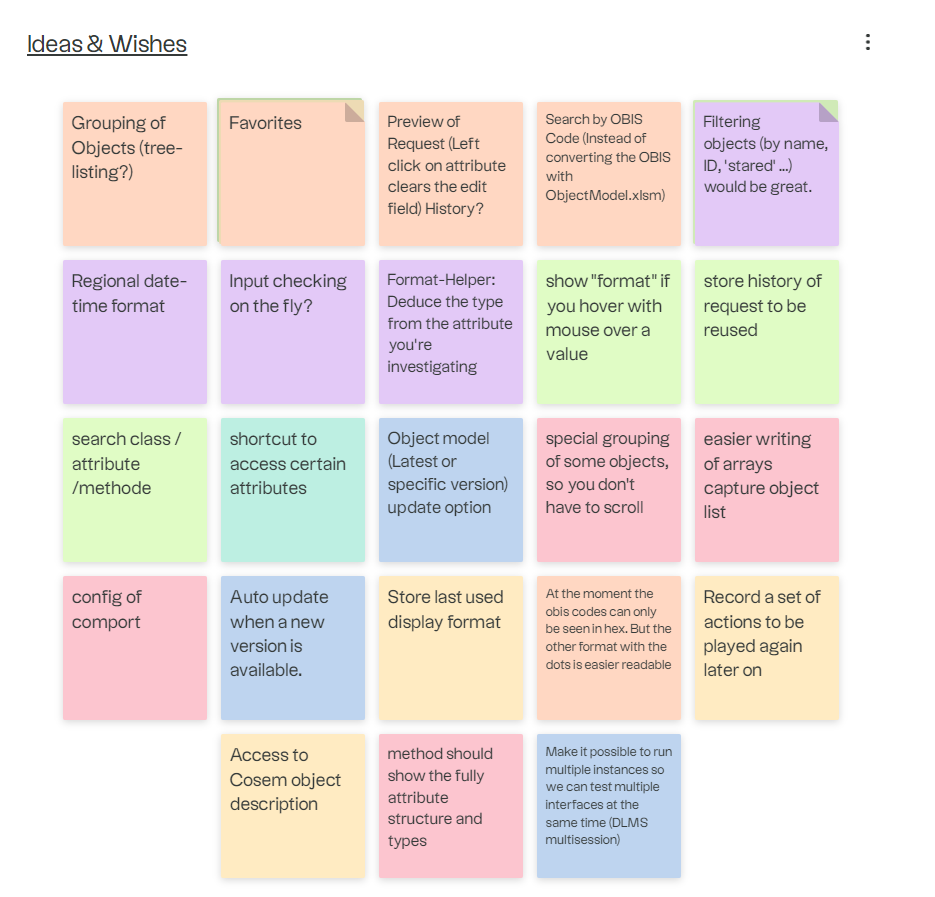
\includegraphics[width=1.0\textwidth]{gfx/S1_RetroBoard_IdeasAndWishes.png}
   \caption{
       Ideen und Wünsche der Nutzer an die neue Anwendung.
   }
   \label{fig:IdeasAndWishes}
\end{figure}

Um die Prioritäten der gesammelten Ideen \& Wünsche herauszufinden, wurde anschliessend an das Meeting eine Umfrage durchgeführt.
Ein Teil dieser Umfrage war es, dass die Nutzer zehn mögliche Features, welche auf den von ihnen eingebrachten Ideen \& Wünsche basieren, zu priorisieren.


\begin{figure}[H]
   \centering
   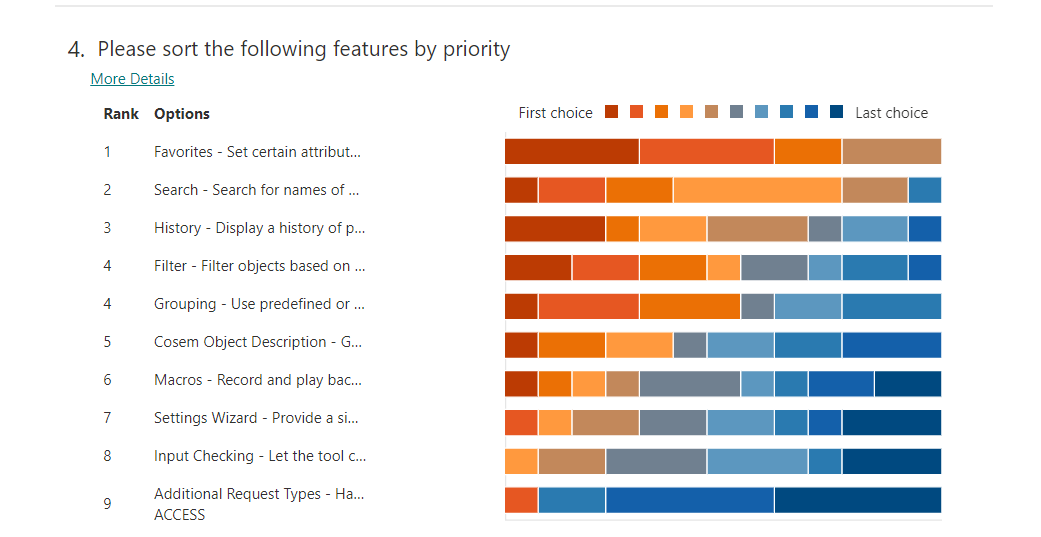
\includegraphics[width=1.0\textwidth]{gfx/S1_Survey_Prio.png}
   \caption{
       Resultat der Umfrage: Sortiere diese Features nach Priorität
   }
   \label{fig:FeaturesPrio}
\end{figure}

Die Nutzer wurden ebenfalls dazu befragt, auf welchen Plattformen sie die neue Anwendung gerne einsetzten würden.
Im nächsten Abschnitt werden die Antworten (Abbildung \ref{fig:SurveryPlatforms}) auf diese Frage sowie viele weitere Aspekte für die Evaluation des Technologiestacks verwendet.

\begin{figure}[H]
   \centering
   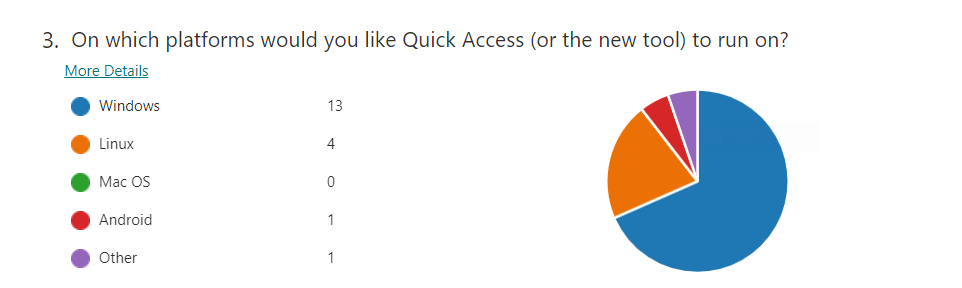
\includegraphics[width=1.0\textwidth]{gfx/S0_Survey_Platform.png}
   \caption{
       Resultat der Umfrage: Gewünschte Plattformen
   }
   \label{fig:SurveryPlatforms}
\end{figure}

\subsection{Evaluation des Technologiestacks}
Um im ersten Sprint mit der Implementation der Applikation beginnen zu können, musste zuerst ein geeigneter Technologiestack evaluiert werden.
Die im vorherigen Abschnitt erwähnt Umfrage hat ergeben, dass sich alle Befragten Windows als Zielplatform der neuen Anwendung wünschen.
Nur vereinzelt wurde nebst Windows noch Android oder Linux angegeben.
Somit
Im Projektauftrag TODO ist festgehalten, dass die Technologien frei gewählt werden können, für die Landis+Gyr jedoch günstig zu unterhalten sein soll.

Um dies zu erreichen, wurden für die Evaluation nur Programmiersprachen in Betracht gezogen, welche bei der Landis+Gyr bereits aktiv verwendet werden.
Im Kapitel \ref{lgintern} werden einige Anwendungen und Softwareprojekte der Landis+Gyr, welche im Umfeld der zu entwickelnden Anwendung betrieben und unterhalten werden, genauer beschrieben.
Die dort verwendeten Programmiersprachen sind C\#, Python und C++.


Ein wichtiger Teil der Anwendung wird die \ac{DLMS} Kommunikation mit den Stromzählern sein.
Diese ist in allen drei zuvor genannten Programmiersprachen bereits implementieren und wird in den Tools \textit{ATS}, \textit{libpydlms} rsp. \textit{DMT2} verwendet.
Da der \textit{DMT2} jedoch von einem externen Lieferanten entwickelt wurde, erlaubt die zugehörige Lizenz die Verwendung des Codes nicht ohne weiteres.


Der Fokus der zu entwickelnden Anwendung liegt auf der Benutzerschnittstelle.
Python Applikationen mit Benutzerschnittstelle gibt es bei der Landis+Gyr keine.
Möglich wäre ein Technologiestack bestehend aus Python Backend mit einem Angular \footnote{https://angular.io} Frontend.
Das Web-Framework Angular, welches mit der Sprache TypeScript verwendet wird, wird im Projekt \textit{Test Script Manager} eingesetzt.
Dieses Projekt wird an einem Standort ausserhalb der Schweiz entwickelt.
Als Backend wird dort jedoch nicht Python sondern C\# eingesetzt.
Eine Python+Angular Applikation wäre somit nicht komplett neu für die Landis+Gyr.

Im Gegensatz zu Python existieren bei der Landis+Gyr bereits mehrere C\# Anwendungen, welche über eine Benutzerschnittstelle verfügen.
Die \textit{PicParted} und \textit{DocTool} sind C\# Anwendungen welche über eine \ac{WPF}\footnote{https://docs.microsoft.com/en-us/visualstudio/designers/getting-started-with-wpf?view=vs-2022} Benutzerschnittstelle verfügen.
Sie werde im Bereich des Picasso Projekts TODO eingesetzt und Unterhalten. 
Ursprünglich wurden sie vom Autor dieser Arbeit entwickelt.

Die Anwendung \textit{ATS}, welche im Abschnitt \ref{ats} genauer beschrieben wird, verfügt über Code für die \ac{DLMS} Kommunikation mit Stromzählern.
Dieser könnte für die neue Anwendung wiederverwendet werden.
Die in Abschnitt \ref{objectModelsClassDescriptions} beschriebenen Tools verfügen ebenfalls über C\# Code, welcher thematisch nahe an der neuen Anwendung ist und evtl. ebenfalls wiederverwendet werden kann.

Aufgrund der genannten Umstände viel die Entscheidung auf einen C\# Technologiestack.

% TODO WinUI3 Evaluation beschreiben

Um im ersten Sprint direkt mit der Entwicklung loslegen zu können wurde in \ac{ADO} ein Repository erstellt.
Dieses wurde mit einer leeren WinUI3 Projekt initialisiert.




\subsection{Erstellung des Backlogs}
Wie in Abschnitt \ref{methoden:ADO} erklärt, wurde \ac{ADO} für die Verwaltung des Backlogs verwendet.
Dazu musste als erstes eine neues \ac{ADO} Projekt erstellt und die Sprints eingetragen werden.
Nun konnten User Stories formuliert und auf die sechs geplanten Sprints verteilt werden.
Welche Stories im ersten Sprint bearbeitet wurden und wie dies genau ablief ist im folgenden Kapitel zu lesen.
% TODO no chli meh schribe?